\section{Analysis}

Consider an execution of the \poem protocol.
We define a discrete and uniformly random variable $X_{r, i}$ as follows.
If at round $r$, honest party $P_i$ finds PoW block $B$, then $X_{r, i} = \work(B)$.
If no PoW was found, $X_{r, i} = 0$.

We define $X_{r}$ as the maximum PoW intrinsic work found by an honest party during
round $r$. Hence, $X_{r} = \max_{i = 1}^{n - t}{X_{r,i}}$.

%TODO: Make the conjecture formal.
\begin{conjecture}[\poem is Secure]
  For all PPT adversaries, the \poem protocol, in
  the static setting, utilizing a synchronous communication network, is
  secure except with negligible probability in the security parameter $\kappa$.
\end{conjecture}

\begin{figure}[h]
    \centering
    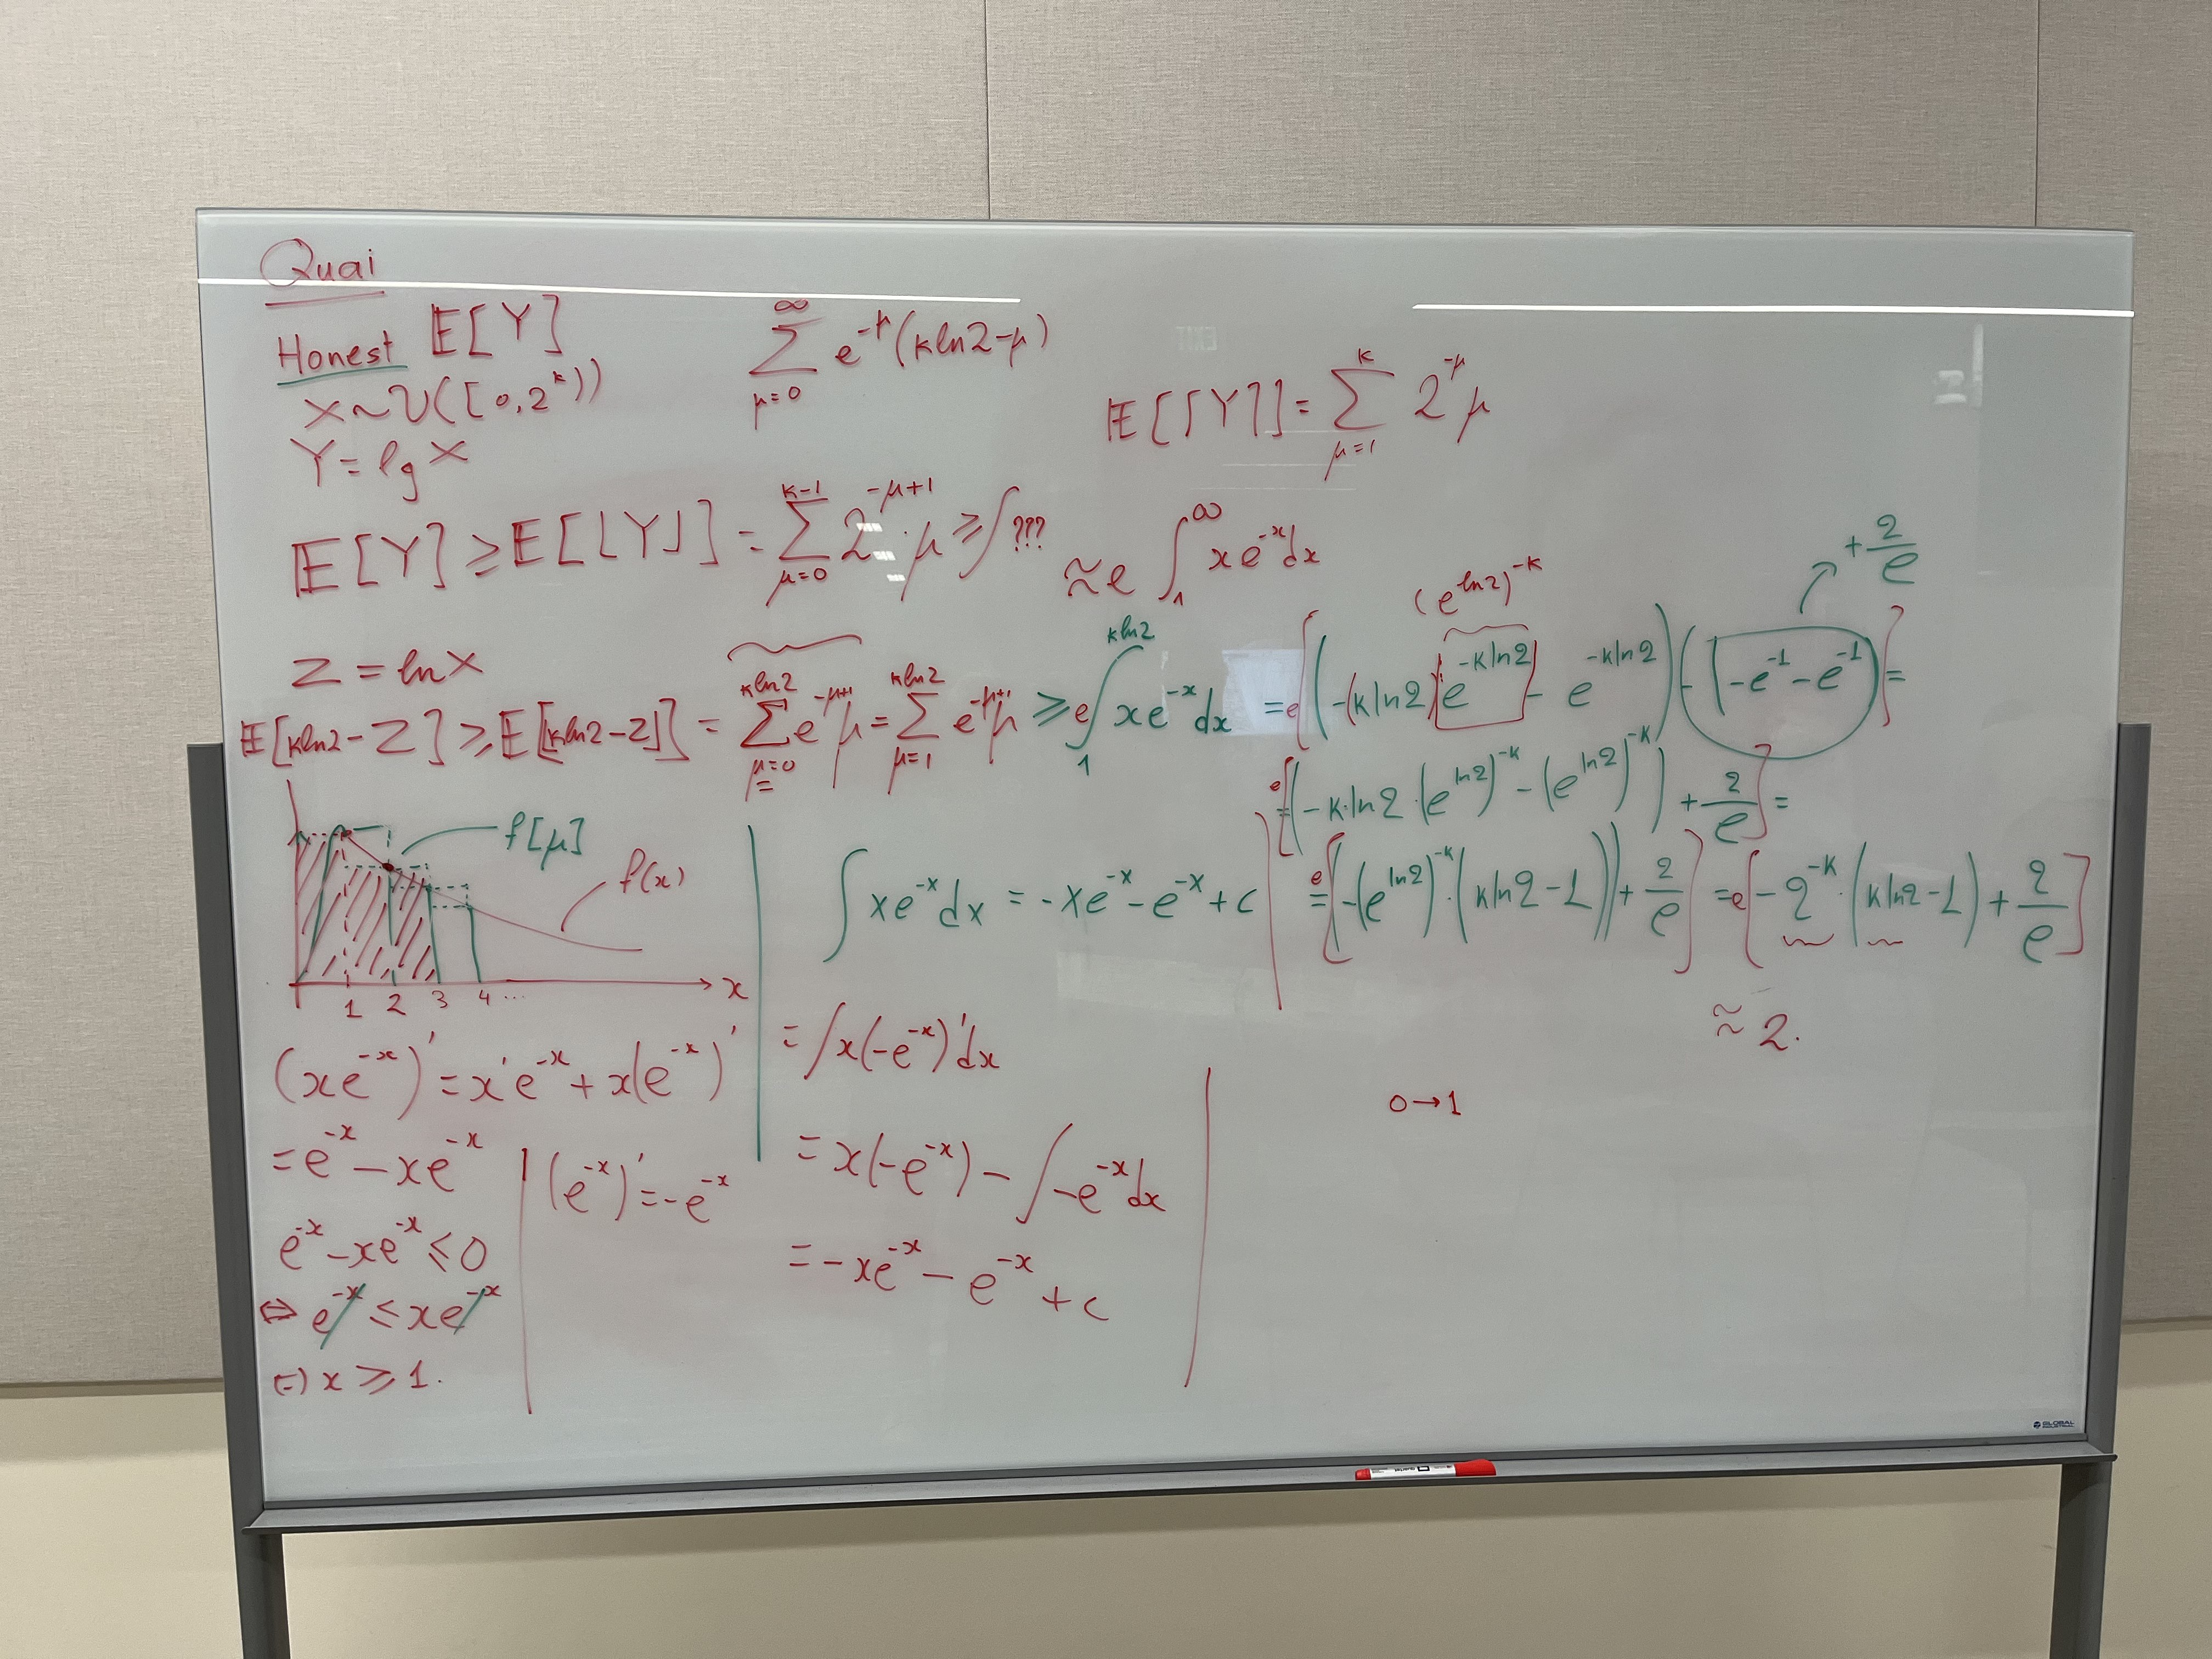
\includegraphics[width=1\textwidth]{figures/bounds-1.jpeg}
\end{figure}

\begin{figure}[h]
    \centering
    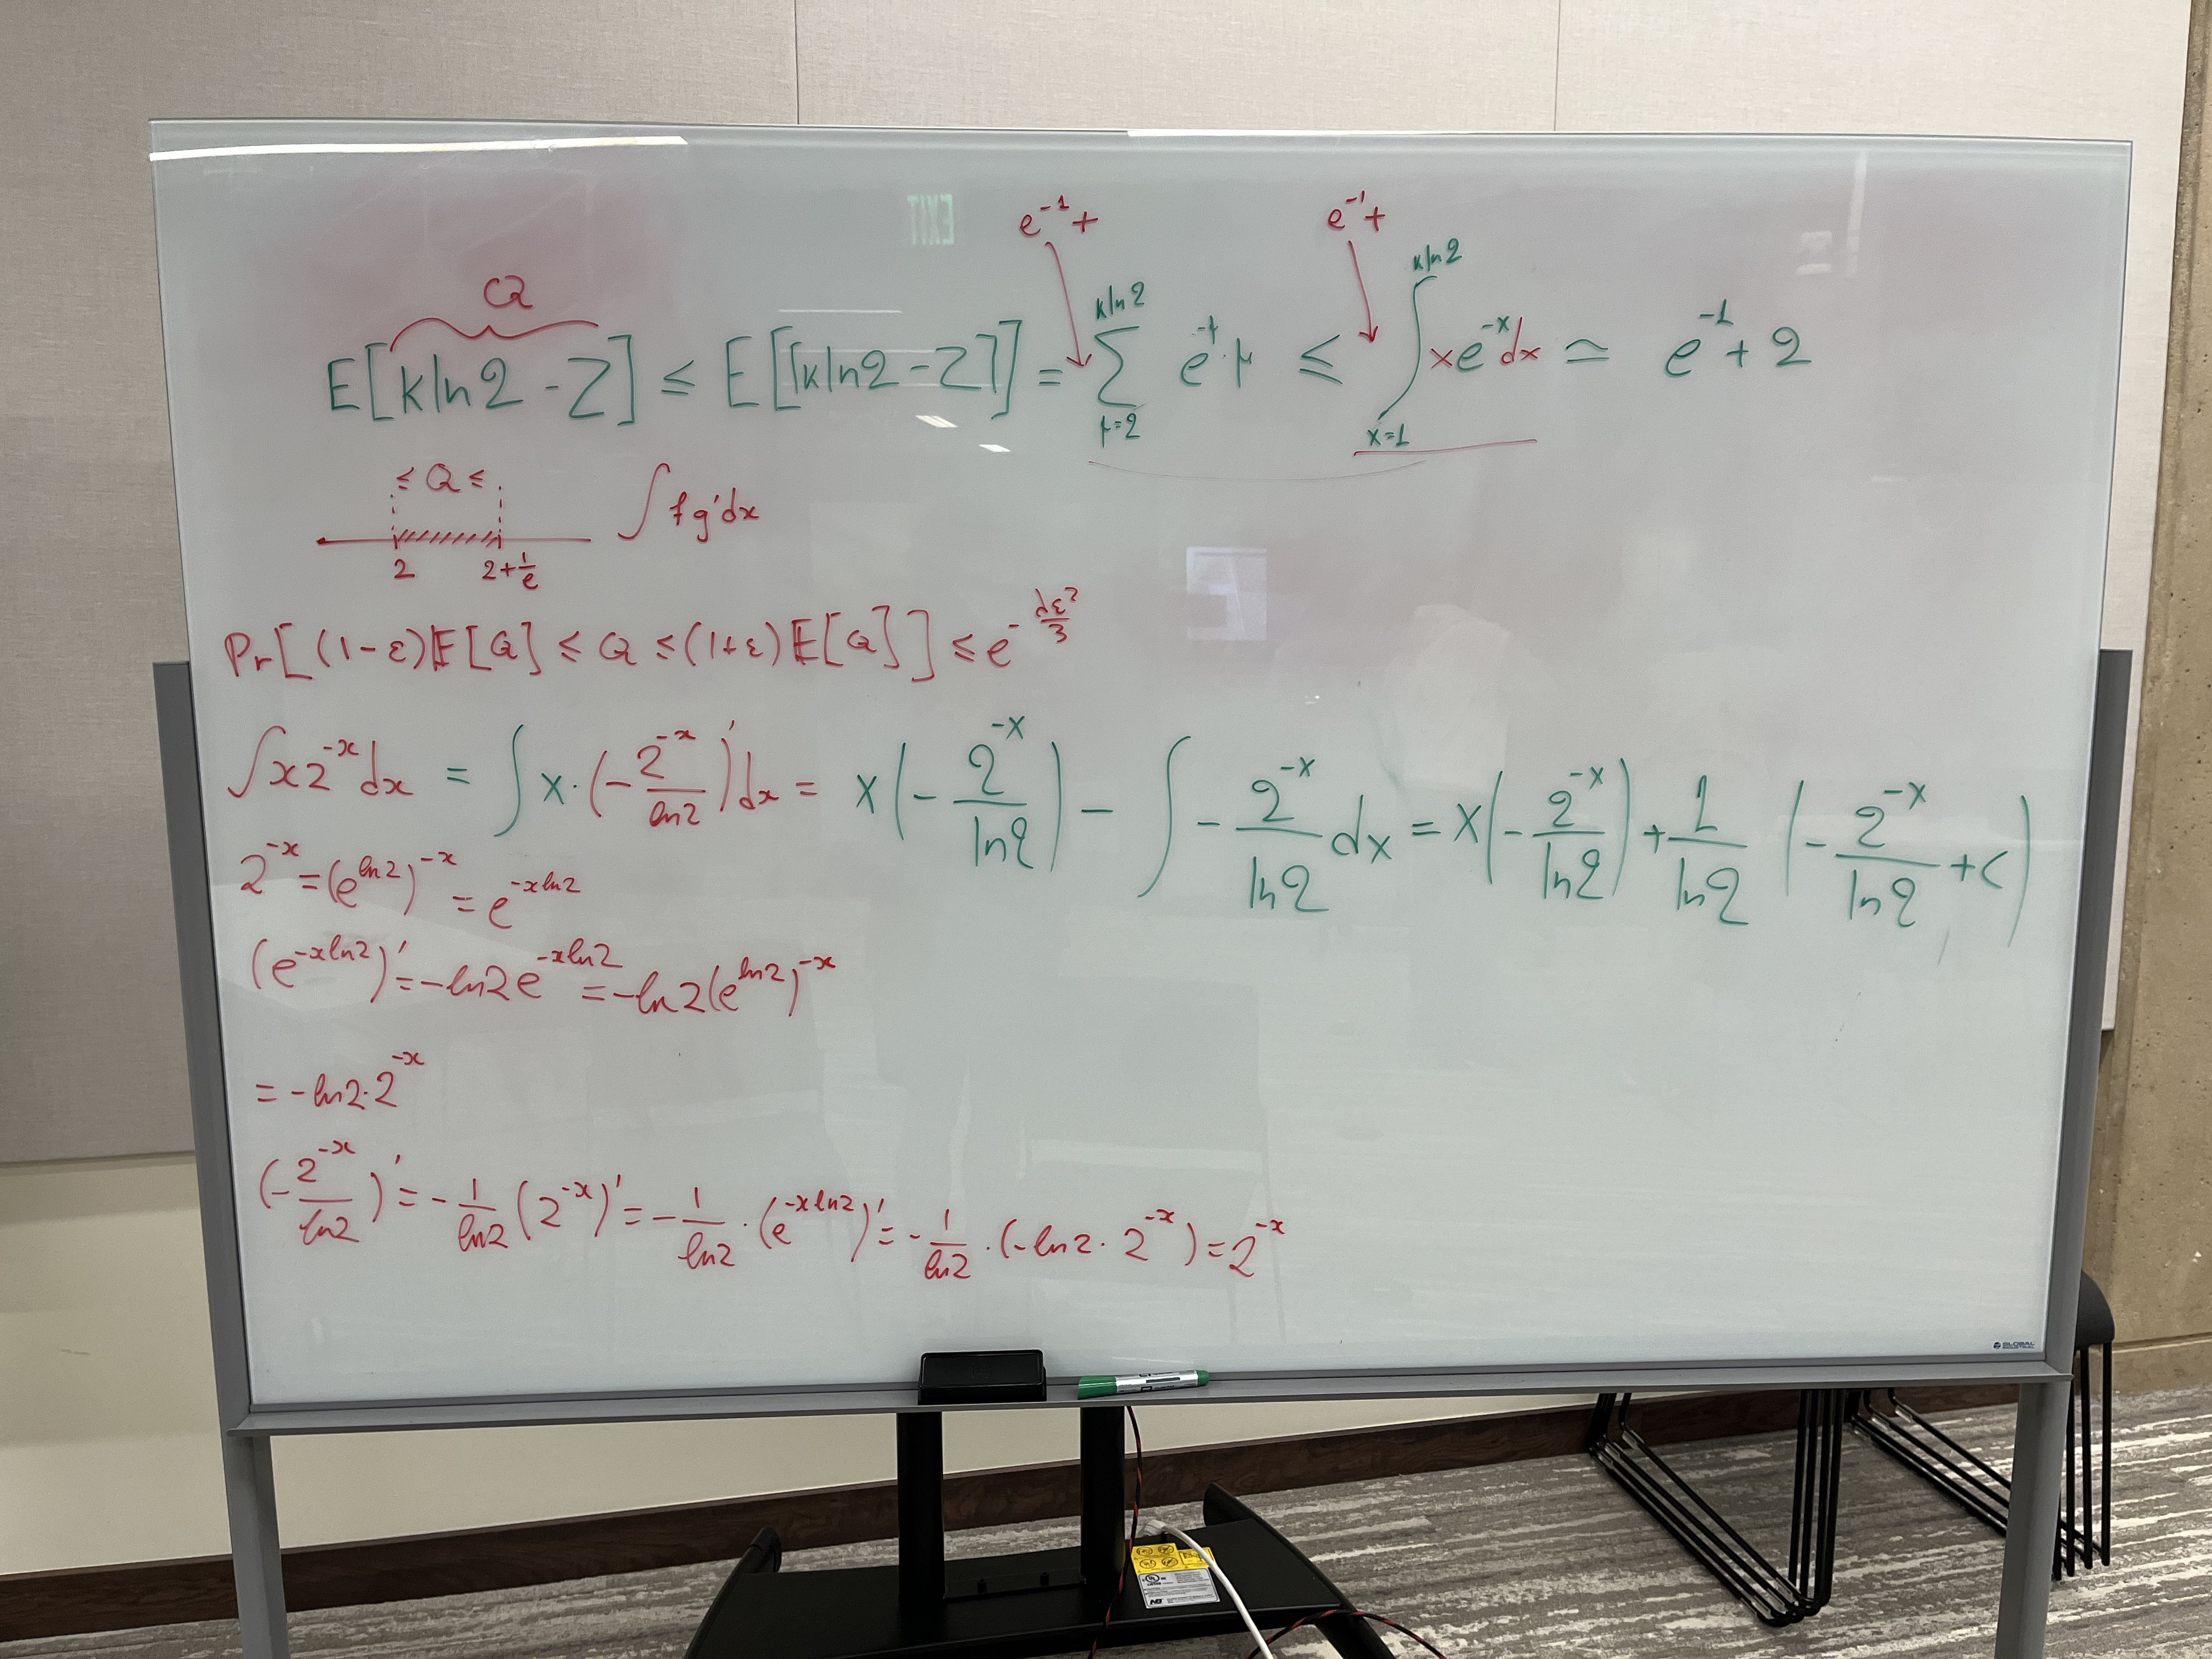
\includegraphics[width=1\textwidth]{figures/bounds-2.jpeg}
\end{figure}
